\section{Introduction}
\label{sec:introduction}



\subsection{Difference Logic}
DL is a special case of an LA logic in which
all LA constraints have the form $ x - y \prec c $ where
$ x $ and $ y $ are numerical variables, $ c $ is a constant
and $ \prec \in \{<, \leq \} $ is a comparison operator.
A more formal definition of DL is given
below~\cite{cotton2004some},~\cite[p.5]{mahfoudh2003verification}:
\begin{definition}[Difference Logic]
    \label{def:differenceLogic}
    Let $ \mathcal{B} = \{ b_1, b_2, \dots \} $ be a set of Boolean
    variables and $ \mathcal{X} = \{ x_1, x_2, \dots \} $ be a set
    of numerical variables. The difference logic over
    $ \mathcal{B} $ and $ \mathcal{X} $ is called
    $ DL(\mathcal{X},\mathcal{B}) $ and given by the following grammar:
    \begin{equation*}
        \phi \eqbydef b \; | \; (x - y < c) \; | \; \neg \phi \; | \;
        \phi \land \phi
    \end{equation*}
    where $ b \in \mathcal{B} $, $ x,y \in \mathcal{X} $ and
    $ c \in \mathbb{D} $ is a constant. The domain $ \mathbb{D} $ is
    either the integers $ \mathbb{Z} $ or the real numbers $ \mathbb{R} $.
    \\
    The remaining Boolean connectives
    $ \lor, \rightarrow, \leftrightarrow, \dots $ can be defined in
    the usual ways in terms of conjunction and negation.
\end{definition}
Examples of DL formulas are given below:
% TODO: add two more examples and use them further in the report
\begin{equation}
    \label{eq:example-1}
    \phi_1 = (p \lor q \lor r) \land (p \rightarrow (u - v < 3)) \land
    (q \rightarrow (v - w < -5)) \land (r \rightarrow (w - x < 0))
\end{equation}
\begin{equation}
    \label{eq:example-2}
    \phi_2 = (a) \land (b)
\end{equation}
\begin{equation}
    \label{eq:example-3}
    \phi_3 = (c)
\end{equation}



\subsection{Solving SAT Problem of Propositional Logic}
Most of the SAT solvers employ a variation of the
Davis-Putnam-Logemann-Loveland (DPLL)
algorithm~\cite{davis1960computing, davis1962machine}
for solving SAT problem of the propositional logic (PL).
One such basic SAT checking algorithm is given below:
\begin{Algorithm}
    \caption{A basic SAT checking algorithm for solving SAT problem of PL.
        It takes a PL formula to be checked for satisfiability and
        returns SAT status of the formula (SAT or UNSAT)
        and, in case when the formula is SAT, a model \ie an assignment, which evaluates the formula to $ True $.}
    \label{alg:basic-sat}
    \begin{algorithm}{\text{(SAT Status, Model) Check}}
        {\text{PL formula} \phi}
        model \= \varnothing \\
        (inferredAssignments, conflictingClauses) \= \CALL{Propagate}(\phi, model) \\
        conflictHasArisen \= conflictingClauses \neq \varnothing \\
        \begin{IF}{conflictHasArisen}
            \RETURN (UNSAT, \NIL)
        \end{IF} \\
        model\=model \cup inferredAssignments \\
        \begin{WHILE}{True}
            (nextVariable, value) \= \CALL{Decide}(\phi, model) \\
            allVariablesHaveAlreadyBeenAssigned \= nextVariable = \NIL \\
            \begin{IF}{allVariablesHaveAlreadyBeenAssigned}
                \RETURN (SAT, model)
            \end{IF} \\
            model \= model \cup \{ nextVariable \= value \} \\
            \begin{REPEAT} \\
                (inferredAssignments, conflictingClauses) \= \CALL{Propagate}(\phi, model) \\
                model \= model \cup inferredAssignments \\
                conflictHasArisen \= conflictingClauses \neq \varnothing \\
                \begin{IF}{conflictHasArisen}
                    (newModelWithoutConflict, \phi_a) \= \CALL{Resolve}(\phi, model, conflictingClauses) \\
                    conflictHasNotBeenResolved \= newModelWithoutConflict = \NIL \\
                    \begin{IF}{conflictHasNotBeenResolved}
                        \RETURN (UNSAT, \NIL)
                    \end{IF} \\
                model \= newModelWithoutConflict \\
                \phi \= \phi \land \phi_a
                \end{IF}
            \end{REPEAT} \neg conflictHasArisen
        \end{WHILE}
    \end{algorithm}
\end{Algorithm}

The given above Algorithm~\ref{alg:basic-sat} is quite generic,
it is more of a template.
One needs to plug into this template his own implementations of the
following functions:
\begin{itemize}
    \item[$ \algCALL{Propagate} $] This function takes a PL formula
    and a model and returns all assignments that follow from
    them.
    It also returns a list of conflicting clauses (if there are any).
    These clauses will be in conflict with the model if one extends
    the model by applying the returned assignments.
    A couple of examples are given below:
    \begin{equation}
        \begin{aligned}
            \phi = a \land b \land (c \lor d) \\
            model = \varnothing \\
            \algCALL{Propagate}(\phi, model)
            = (\{ a = True, b = True \}, \varnothing) \\
        \end{aligned}
    \end{equation}
    \begin{equation}
        \begin{aligned}
            \phi = (a \lor b \lor c) \land (\neg c \lor d)
                \land (\neg d \lor a \lor e) \\
            model = \{ a = False, b = False \} \\
            \algCALL{Propagate}(\phi, model)
                = (\{ c = True, d = True, e = True \}, \varnothing) \\
        \end{aligned}
    \end{equation}
    \begin{equation}
        \begin{aligned}
            \phi = (a \lor b \lor c) \land (\neg c \lor d)
                \land (\neg d \lor a) \\
            model = \{ a = False, b = False \} \\
            \algCALL{Propagate}(\phi, model)
                = (\{ c = True, d = True \}, \{ (\neg d \lor a) \}) \\
        \end{aligned}
    \end{equation}
    \item[$ \algCALL{Decide} $] This function takes a PL formula
    and a model and, by applying some heuristic, selects a variable and a
    value for it and returns them.
    The returned variable and value describe an update to the model.
    They basically correspond to a subtree in which the $ \algCALL{Check} $
    algorithm should look for the solution.
    The whole tree represents the model space.
    The leaves of the tree correspond to particular models.
    If all variables in the model have been already assigned the
    function should return $ \algNIL $ as the next variable.
    An example is given below:
    \begin{figure}[htb]
        \begin{center}
            \begin{tabular}{cc}
                \begin{minipage}{0.45\linewidth}
                    \begin{center}
                        \begin{equation}
                        \label{eq:decide-example}
                        \begin{aligned}
                            \phi = (a \lor \neg b \lor c) \lor (b \lor \neg c \lor \neg a) \\
                            model = \{ a = True \} \\
                            \algCALL{Decide}(\phi, model) = (b, False) \\
                        \end{aligned}
                        \end{equation}
                    \end{center}
                \end{minipage}
                &
                \begin{minipage}{0.50\linewidth}
                    \begin{center}
                        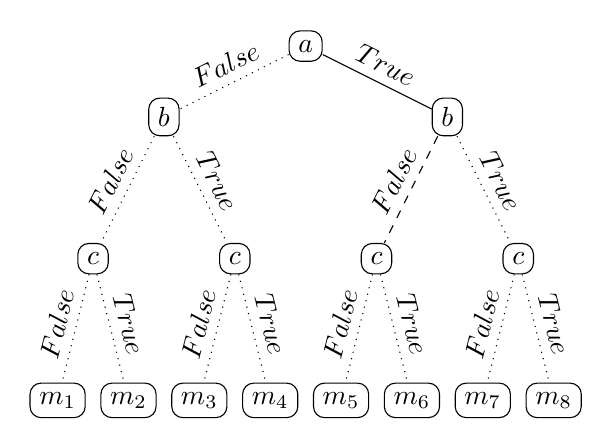
\begin{tikzpicture}[scale=0.9,state/.style={draw, rounded corners, fill=none,text centered, text=black}]
    \node[state] (n1) at (3.5, 5) {$a$};

    \node[state] (n2) at (1.5, 4) {$b$};
    \node[state] (n3) at (5.5, 4) {$b$};
    
    \node[state] (n4) at (0.5, 2) {$c$};
    \node[state] (n5) at (2.5, 2) {$c$};
    \node[state] (n6) at (4.5, 2) {$c$};
    \node[state] (n7) at (6.5, 2) {$c$};

    \node[state] (n8) at (0, 0) {$m_1$};
    \node[state] (n9) at (1, 0) {$m_2$};
    \node[state] (n10) at (2, 0) {$m_3$};
    \node[state] (n11) at (3, 0) {$m_4$};
    \node[state] (n12) at (4, 0) {$m_5$};
    \node[state] (n13) at (5, 0) {$m_6$};
    \node[state] (n14) at (6, 0) {$m_7$};
    \node[state] (n15) at (7, 0) {$m_8$};

    \path[every node/.style={sloped,anchor=south,auto=false}]
        (n1) edge[dotted] node {$False$} (n2)
        (n1) edge node {$True$} (n3)

        (n2) edge[dotted] node {$False$} (n4)
        (n2) edge[dotted] node {$True$} (n5)
        (n3) edge[dashed] node {$False$} (n6)
        (n3) edge[dotted] node {$True$} (n7)

        (n4) edge[dotted] node {$False$} (n8)
        (n4) edge[dotted] node {$True$} (n9)
        (n5) edge[dotted] node {$False$} (n10)
        (n5) edge[dotted] node {$True$} (n11)
        (n6) edge[dotted] node {$False$} (n12)
        (n6) edge[dotted] node {$True$} (n13)
        (n7) edge[dotted] node {$False$} (n14)
        (n7) edge[dotted] node {$True$} (n15);
\end{tikzpicture}

                    \end{center}
                \end{minipage}
            \end{tabular}
        \end{center}
        \caption{A example of a decision over a PL formula
            (Equation~\ref{eq:decide-example} on the left)
            and the corresponding model space (on the right).
            The solid edge from $ a $ to $ b $ corresponds to the current
            model ($ model $ in~Equation~\ref{eq:decide-example}).
            The dashed edge from $ b $ to $ c $ corresponds to the decision
            $ (b, False) $ returned by the $ \algCALL{Decide}(\phi, model) $.
            The leaves $ m_1, m_2, \dots, m_8 $ correspond to models \eg $ m_3 $ corresponds to the model $ \{ a=False, b=True, c=False \} $.}
    \end{figure}
    \item[\algCALL{Resolve}] This function takes a PL formula, current
    conflicting model and a list of the clauses which are in the conflict
    with the current model.
    It returns a new model which does not have the conflict and an assertion clause
    $ \phi_a $ (or a conjunction of assertion clauses) which carries the knowledge
    about the resolved conflict.
    The assertion clause evaluates to $ False $ when the same model is used that caused
    the conflict.
    It causes the updated PL formula ($ \phi \land \phi_a $) to also evaluate
    to $ False $ and makes sure the solver will not run into this
    particular conflict again.
    The function should also make sure that the returned conflict-free model
    should be distinct from the models, which have already been processed before.
    Otherwise, the algorithm might fall into an infinite loop.
    If the conflict cannot be resolved, the function returns $ \algNIL $ as
    the model.
    An example is given below:
    \begin{equation}
        \begin{aligned}
            \phi = (a \lor b \lor c) \land (\neg c \lor d) \land (\neg d \lor a) \\
            model = \{ a = False, b = False, c = True, d = True \} \\
            conflictingClauses = \{ (\neg d \lor a) \} \\
            \begin{split}
                \algCALL{Resolve}(\phi, model, conflictingClauses) = \\
                & ( \; \{ a = False \}, \; \{ (a \lor b) \} \; )
            \end{split} \\
        \end{aligned}
    \end{equation}
\end{itemize}

In the described above Algorithm~\ref{alg:basic-sat} a model is represented by
a mapping from PL variables of the input PL formula to booleans.
It is a simplification.
Real SAT solvers maintain a lot of additional information such as decision
levels, assignment order of variables for every decision level, an implicant for
every variable (\ie the clause from which the variable's value was inferred during
the $ \algCALL{Propagate} $) \etc



\subsection{Solving SAT Problem of Difference Logic}
As mentioned in~\cite{cotton2004some} the following main approaches are used for
solving the SAT problem of DL:
\begin{itemize}
    \item Lazy approach. The input DL formula is transformed into
    \item Preprocessing approach.
    \item Incremental approach. test
\end{itemize}